\documentclass[border=10pt]{standalone}

\usepackage{tikz}
\usepackage{tikzsymbols}
\usetikzlibrary{calc,patterns,shapes.geometric}

\def\centerarc[#1](#2)(#3:#4:#5){\draw[#1] ($(#2)+({#5*cos(#3)},{#5*sin(#3)})$) arc (#3:#4:#5);}

\begin{document}
	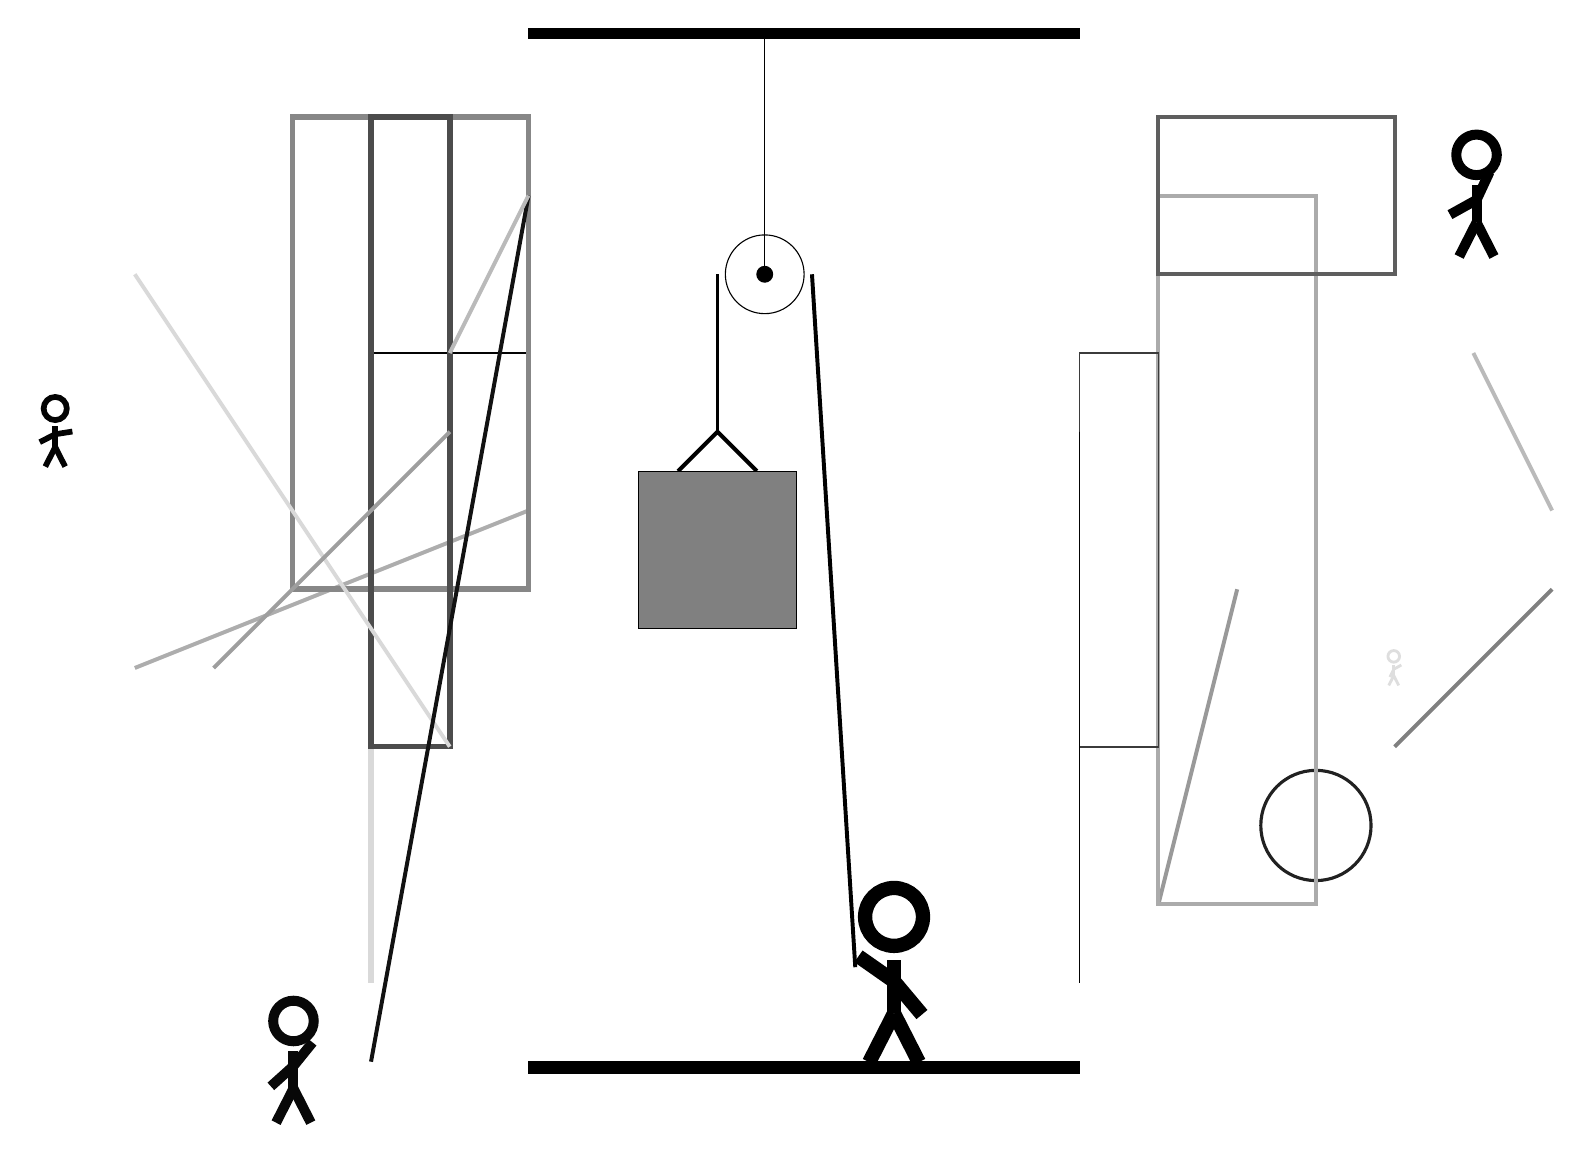
\begin{tikzpicture}
		%%%%% START %%%%%
		
		\draw[fill=black] (-2, 10) rectangle (5, 10.125);
		
		\draw (1, 7) circle (0.5);
		\draw[fill=black] (1, 7) circle (0.1);
		\draw (1, 10) -- (1, 7);
		
		\draw[line width=0.5mm] (-0.1, 4.5) -- (0.4, 5.0) -- (0.9, 4.5);
		\draw[fill=black!50] (-0.6, 4.5) rectangle (1.4, 2.5);
		
		\draw[line width=0.5mm] (0.4, 7) -- (0.4, 5.0);
		\centerarc[line width=0.5mm](1, 7)(0:180:0.6);
		\draw[line width=0.5mm](1.6, 7) -- (2.15, -1.8);
		
		\node at (2.6, -1.9) {\Strichmaxerl[10][-35][-50]};
		
		\draw[line width=0.2mm, color=black!99] (-4, 3) rectangle (-2, 6);
		
		\draw[line width=0.5mm, color=black!32](-7, 2) -- (-2, 4);
		\draw[line width=0.5mm, color=black!40](7, 3) -- (6, -1);
		\node[line width=0.3mm, color=black!99] at (-8, 5) {\Strichmaxerl[4][27][9]};
		
		\draw[line width=0.7mm, color=black!15] (-4, -2) rectangle (-4, 2);
		\draw [line width=0.4mm, color=black!87](8, 0) circle (0.7);
		\draw[line width=0.5mm, color=black!33] (6, -1) rectangle (8, 8);
		\draw[line width=0.7mm, color=black!47] (-2, 3) rectangle (-5, 9);
		\node[line width=0.6mm, color=black!100] at (10, 8) {\Strichmaxerl[7][29][65]};
		
		\draw[line width=0.5mm, color=black!27](10, 6) -- (11, 4);
		\draw[line width=0.7mm, color=black!70] (-4, 1) rectangle (-3, 9);
		
		\draw[line width=0.5mm, color=black!15](-3, 1) -- (-7, 7);
		\draw[line width=0.5mm, color=black!38](-3, 5) -- (-6, 2);
		
		\node[line width=0.4mm, color=black!13] at (9, 2) {\Strichmaxerl[2][64][29]};
		\draw[line width=0.5mm, color=black!63] (6, 7) rectangle (9, 9);
		\node[line width=0.6mm, color=black!97] at (-5, -3) {\Strichmaxerl[7][42][51]};
		\draw[line width=0.2mm, color=black!77] (6, 1) rectangle (5, 6);
		\draw[line width=0.2mm, color=black!99] (5, -2) rectangle (5, 5);
		\draw[line width=0.5mm, color=black!50](9, 1) -- (11, 3);
		
		\draw[line width=0.5mm, color=black!93](-4, -3) -- (-2, 8);
		\draw[line width=0.5mm, color=black!27](-2, 8) -- (-3, 6);
		
		\draw[fill=black] (-2, -3) rectangle (5, -3.15);
		
		%%%%% END %%%%%
	\end{tikzpicture}
\end{document}